%*************************************************************************
% A Classic Thesis Style
% An Homage to The Elements of Typographic Style
%
% Copyright (C) 2017 André Miede and Ivo Pletikosić
%
% If you like the style then I would appreciate a postcard. My address
% can be found in the file ClassicThesis.pdf. A collection of the
% postcards I received so far is available online at
% http://postcards.miede.de
%
% License:
% This program is free software; you can redistribute it and/or modify
% it under the terms of the GNU General Public License as published by
% the Free Software Foundation; either version 2 of the License, or
% (at your option) any later version.
%
% This program is distributed in the hope that it will be useful,
% but WITHOUT ANY WARRANTY; without even the implied warranty of
% MERCHANTABILITY or FITNESS FOR A PARTICULAR PURPOSE.  See the
% GNU General Public License for more details.
%
% You should have received a copy of the GNU General Public License
% along with this program; see the file COPYING.  If not, write to
% the Free Software Foundation, Inc., 59 Temple Place - Suite 330,
% Boston, MA 02111-1307, USA.
%
% PLEASE SEE ALSO THE AUTHORS' NOTE REGARDING THIS LICENSE
% IN THE DOCUMENTATION (ClassicThesis.pdf --> Chapter 1 / Chapter01.tex)
%*************************************************************************
\RequirePackage{silence} % :-\
    \WarningFilter{scrreprt}{Usage of package `titlesec'}
    %\WarningFilter{scrreprt}{Activating an ugly workaround}
    \WarningFilter{titlesec}{Non standard sectioning command detected}
\documentclass[ openright,titlepage,numbers=noenddot,headinclude,%twoside, %1headlines,% letterpaper a4paper
                footinclude=true,cleardoublepage=empty,abstractoff, % <--- obsolete, remove (todo)
                BCOR=5mm,paper=a4,fontsize=11pt,%11pt,a4paper,%
                ngerman,american,%lockflag%
                ]{scrreprt}

%*************************************************************************
% Note: Make all your adjustments in here
%*************************************************************************
% ****************************************************************************************************
% hdathesis-config.tex 
% Use it at the beginning of your thesis.tex, or as a LaTeX Preamble 
% in your thesis.{tex,lyx} with % ****************************************************************************************************
% hdathesis-config.tex 
% Use it at the beginning of your thesis.tex, or as a LaTeX Preamble 
% in your thesis.{tex,lyx} with % ****************************************************************************************************
% hdathesis-config.tex 
% Use it at the beginning of your thesis.tex, or as a LaTeX Preamble 
% in your thesis.{tex,lyx} with \input{hdathesis-config}
% ****************************************************************************************************

% ****************************************************************************************************
% 1. Personal data and user ad-hoc commands
% ****************************************************************************************************
\newcommand{\myTitle}{Bewertung verschiedener Technologien zur Abwehr von Bot-Angriffen und ihr Einfluss auf die Nutzererfahrung\xspace}
%\newcommand{\mySubtitle}{An Homage to The Elements of Typographic Style\xspace}
\newcommand{\myDegree}{Bachelor of Science (B.Sc.)\xspace} 
%\newcommand{\myDegree}{Bachelor of Arts (B.A.)\xspace}
%\newcommand{\myDegree}{Master of Science (M.Sc.)\xspace}
%\newcommand{\myDegree}{Master of Arts (M.A.)\xspace}
\newcommand{\myName}{Tessa-Mae Victoria Leps\xspace}
\newcommand{\myId}{760240\xspace}
\newcommand{\myProf}{Prof. Dr. Stefan Zander\xspace}
\newcommand{\myOtherProf}{Prof. Dr. Daniel Burda\xspace}
\newcommand{\myFaculty}{Fachbereich Informatik\xspace}
\newcommand{\myUni}{Hochschule Darmstadt\xspace}
\newcommand{\myLocation}{Darmstadt\xspace}
\newcommand{\myTime}{25. August 2022\xspace}
\newcommand{\myVersion}{version 4.4\xspace}

% ****************************************************************************************************
% 2. Is it a master thesis?
% ****************************************************************************************************
%\PassOptionsToPackage{master}{hdahesis} % uncomment if this is a master thesis 

% ****************************************************************************************************
% 3. Does the thesis have a lock flag?
% ****************************************************************************************************
%\PassOptionsToPackage{lockflag}{hdathesis} % uncomment if this thesis has a lock flag 

% ****************************************************************************************************
% 4. Loading some handy packages
% ****************************************************************************************************
% ****************************************************************************************************
% Packages with options that might require adjustments
% ****************************************************************************************************

%\PassOptionsToPackage{ngerman,american}{babel}   % change this to your language(s)
% Spanish languages need extra options in order to work with this template
%\PassOptionsToPackage{spanish,es-lcroman}{babel}
\usepackage{babel}


% ****************************************************************************************************

% ****************************************************************************************************
% 1. Personal data and user ad-hoc commands
% ****************************************************************************************************
\newcommand{\myTitle}{Bewertung verschiedener Technologien zur Abwehr von Bot-Angriffen und ihr Einfluss auf die Nutzererfahrung\xspace}
%\newcommand{\mySubtitle}{An Homage to The Elements of Typographic Style\xspace}
\newcommand{\myDegree}{Bachelor of Science (B.Sc.)\xspace} 
%\newcommand{\myDegree}{Bachelor of Arts (B.A.)\xspace}
%\newcommand{\myDegree}{Master of Science (M.Sc.)\xspace}
%\newcommand{\myDegree}{Master of Arts (M.A.)\xspace}
\newcommand{\myName}{Tessa-Mae Victoria Leps\xspace}
\newcommand{\myId}{760240\xspace}
\newcommand{\myProf}{Prof. Dr. Stefan Zander\xspace}
\newcommand{\myOtherProf}{Prof. Dr. Daniel Burda\xspace}
\newcommand{\myFaculty}{Fachbereich Informatik\xspace}
\newcommand{\myUni}{Hochschule Darmstadt\xspace}
\newcommand{\myLocation}{Darmstadt\xspace}
\newcommand{\myTime}{25. August 2022\xspace}
\newcommand{\myVersion}{version 4.4\xspace}

% ****************************************************************************************************
% 2. Is it a master thesis?
% ****************************************************************************************************
%\PassOptionsToPackage{master}{hdahesis} % uncomment if this is a master thesis 

% ****************************************************************************************************
% 3. Does the thesis have a lock flag?
% ****************************************************************************************************
%\PassOptionsToPackage{lockflag}{hdathesis} % uncomment if this thesis has a lock flag 

% ****************************************************************************************************
% 4. Loading some handy packages
% ****************************************************************************************************
% ****************************************************************************************************
% Packages with options that might require adjustments
% ****************************************************************************************************

%\PassOptionsToPackage{ngerman,american}{babel}   % change this to your language(s)
% Spanish languages need extra options in order to work with this template
%\PassOptionsToPackage{spanish,es-lcroman}{babel}
\usepackage{babel}


% ****************************************************************************************************

% ****************************************************************************************************
% 1. Personal data and user ad-hoc commands
% ****************************************************************************************************
\newcommand{\myTitle}{Bewertung verschiedener Technologien zur Abwehr von Bot-Angriffen und ihr Einfluss auf die Nutzererfahrung\xspace}
%\newcommand{\mySubtitle}{An Homage to The Elements of Typographic Style\xspace}
\newcommand{\myDegree}{Bachelor of Science (B.Sc.)\xspace} 
%\newcommand{\myDegree}{Bachelor of Arts (B.A.)\xspace}
%\newcommand{\myDegree}{Master of Science (M.Sc.)\xspace}
%\newcommand{\myDegree}{Master of Arts (M.A.)\xspace}
\newcommand{\myName}{Tessa-Mae Victoria Leps\xspace}
\newcommand{\myId}{760240\xspace}
\newcommand{\myProf}{Prof. Dr. Stefan Zander\xspace}
\newcommand{\myOtherProf}{Prof. Dr. Daniel Burda\xspace}
\newcommand{\myFaculty}{Fachbereich Informatik\xspace}
\newcommand{\myUni}{Hochschule Darmstadt\xspace}
\newcommand{\myLocation}{Darmstadt\xspace}
\newcommand{\myTime}{25. August 2022\xspace}
\newcommand{\myVersion}{version 4.4\xspace}

% ****************************************************************************************************
% 2. Is it a master thesis?
% ****************************************************************************************************
%\PassOptionsToPackage{master}{hdahesis} % uncomment if this is a master thesis 

% ****************************************************************************************************
% 3. Does the thesis have a lock flag?
% ****************************************************************************************************
%\PassOptionsToPackage{lockflag}{hdathesis} % uncomment if this thesis has a lock flag 

% ****************************************************************************************************
% 4. Loading some handy packages
% ****************************************************************************************************
% ****************************************************************************************************
% Packages with options that might require adjustments
% ****************************************************************************************************

%\PassOptionsToPackage{ngerman,american}{babel}   % change this to your language(s)
% Spanish languages need extra options in order to work with this template
%\PassOptionsToPackage{spanish,es-lcroman}{babel}
\usepackage{babel}


\input{classicthesis-config}

%*************************************************************************
% Bibliographies
%*************************************************************************
\addbibresource{bibliography.bib}

%*************************************************************************
% Hyphenation
%*************************************************************************
%\hyphenation{put special hyphenation here}

%*************************************************************************
% GO!GO!GO! MOVE IT!
%*************************************************************************
\begin{document}
\frenchspacing
\raggedbottom
\selectlanguage{ngerman} % ngerman, american
%\renewcommand*{\bibname}{new name}
%\setbibpreamble{}
\pagenumbering{roman}
\pagestyle{plain}
%*************************************************************************
% Frontmatter
%*************************************************************************
\include{frontbackmatter/Titlepage}
\include{frontbackmatter/Titleback}
%\cleardoublepage\include{frontbackmatter/Dedication}
%\cleardoublepage\include{frontbackmatter/Foreword}
\cleardoublepage\include{frontbackmatter/Declaration}
\condLOCK{\cleardoublepage\include{frontbackmatter/BlockingNotice}}
\cleardoublepage%*******************************************************
% Abstract in English
%*******************************************************
\pdfbookmark[0]{Abstract}{Abstract}


\begin{otherlanguage}{american}
	\chapter*{Abstract}
	Reducing the usage of resources is essential when maintaining a website. 
	“Completely automated public turing tests to tell computers and humans apart”, in short CAPTCHA, are often used to prevent attacks from malicious bots. 
	The completion of these tests is often complicated and disrupts the usage of the website. 

	In the following paper we look at different techniques to tell humans and computers apart and how they influence the development and usage of websites and their security. 
	
	For this purpose we design an evaluation matrix to rate different methods regarding their simplicity to complete, their accessibility, their technical feasibility and their security. 
	
	Based on this evaluation we look at different fields of use to determine which CAPTCHA method is the best option overall.

	CAPTCHAs with minor amounts of inputs needed from the user, like reCAPTCHA v3 or hCaptcha, score very high in all categories and are a good choice,
	even with emphasis on different aspects.  

	Other CAPTCHAs can also be a solid choice in some cases.

	Some kinds of CAPTCHAs are not used very often in current times. 
	Because of this, they weren't considered any further or scored very low.

\end{otherlanguage}

\cleardoublepage%*******************************************************
% Abstract in German
%*******************************************************
\begin{otherlanguage}{ngerman}
	\pdfbookmark[0]{Zusammenfassung}{Zusammenfassung}
	\chapter*{Zusammenfassung}
	Bei der Betreibung von Webseiten ist das Einsparen von Ressourcen essentiell. 
	Häufig werden dazu „completely automated public turing tests to tell computers and humans apart“ - im Sprachgebrauch meist als CAPTCHA abgekürzt - eingesetzt, um Angriffe durch Bots zu unterbinden. 
	Das Ausfüllen dieser Tests ist oftmals kompliziert und stört den menschlichen Anwender bei der Benutzung.

	In der folgenden Arbeit wird betrachtet, wie sich verschiedene Techniken zur Unterscheidung von Menschen und Maschine auf die Erfahrung bei der Entwicklung und Nutzung von Webseiten sowie deren Schutz auswirken. 
	Hierzu wird eine Bewertungsmatrix entwickelt. 

	Mithilfe dieser Matrix werden ausgewählte Methoden hinsichtlich der Bedienfreundlichkeit bei dem Ausfüllen des Tests, Accessability, technischer Umsetzbarkeit und Sicherheit beurteilt. 
	 
	Anschließend werden - abhängig der Anforderungen verschiedener Einsatzgebiete Empfehlungen - ausgesprochen, welche der Optionen die beste Gesamtleistung bieten.

	CAPTCHAs mit geringem User-Input, wie beispielsweise reCAPTCHA v3 oder hCaptcha, erzielen hohe Bewertungen und sind auch bei vielen verschiedenen Gewichtungen
	eine gute Wahl. 
	Andere Arten von CAPTCHAs können für spezielle Anwendungsgebiete trotzdem eine bessere, oder zumindest gleichwertige, Wahl darstellen.
	
	Einige CAPTCHA-Arten sind heutzutage nicht mehr in Benutzung und wurden deshalb entweder nicht weiter betrachtet,
	oder haben sehr niedrige Scores erreicht.

\end{otherlanguage}

%\cleardoublepage\include{frontbackmatter/Publications}
%\cleardoublepage\include{frontbackmatter/Acknowledgments}
\cleardoublepage\include{frontbackmatter/Contents}
\cleardoublepage\include{frontbackmatter/Figures}
\cleardoublepage\include{frontbackmatter/Tables}
\cleardoublepage\include{frontbackmatter/Listings}
\cleardoublepage\include{frontbackmatter/Acronyms}
%*************************************************************************
% Mainmatter
%*************************************************************************
\cleardoublepage
\pagestyle{scrheadings}
\pagenumbering{arabic}
% Alwas use \cleardoublepage before \part{...}.
\cleardoublepage
\part{Thesis}\label{pt:thesis}
\chapter{Einleitung}
\label{ch:intro}

Für die Unterscheidung von Menschen und Maschine bei der Betreibung von Webseiten werden verschiedene Methoden genutzt.
Eine davon sind sogenannte CAPTCHA - ``completely automated turing tests to tell computers and humans apart''.
Besonders wenn es um das Ausfüllen von Anmelde- oder Bestellformularen geht, sind diese häufig anzutreffen.

Das Ausfüllen von CAPTCHAs unterbricht oftmals die normale Nutzung von Webseiten und kann als störend empfunden werden.

Ihre Nutzung ist notwendig, um übermäßige Belastungen von Webseiten und den Missbrauch fremder Daten einzudämmen oder ganz zu verhindern.
Es soll also verhindert werden, dass Seiten oder Dienste durch Bots missbraucht werden.

Um die Nutzererfahrung so angenehm wie möglich gestalten zu können,
muss sorgfältig abgewägt werden, welcher CAPTCHA eingesetzt werden sollte. 

Aus diesem Grund soll eine Möglichkeit geschaffen werden, um CAPTCHAs und ihre Alternativen bewerten zu können.
%\section{Motivation}
%\label{sec:intro:motivation}


%
% Section: Ziele
%
\section{Ziel der Arbeit}
\label{sec:intro:goal}

Ziel der Arbeit ist es, eine Bewertungsmatrix für CAPTCHA-Technologien zu bieten, welche bei der Auswahl einer geeigneten Methode unterstützen soll.
Es sind folgende Leitfragen zu klären:

Kann auf Basis von zuvor gewählten Kategorien eine aussagekräftige Matrix zur
Bewertung verschiedener CAPTCHA-Methoden und ihrer Alternativen entwickeln werden?

Kann auf Basis dieser Matrix und einer gegebenen Gewichtung
ein aussagekräftiger Score für bestimmte Einsatzgebiete berechnet werden?

%
% Section: Struktur der Arbeit
%
\section{Gliederung}
\label{sec:intro:structure}
In der folgenden Arbeit werden verschiedene CAPTCHA-Methoden, sowie einige Alternativen zu klassischen CAPTCHAs,
hinsichtlich ihres Einflusses auf die Nutzung von Webseiten betrachtet.

Hierfür wird eine Bewertungsmatrix entwickelt, mithilfe derer die unterschiedlichen Techniken basierend auf
ihrer Bedienfreundlichkeit beim Ausfüllen, ihrer Accessibility, der technischen Umsetzbarkeit $($Implementation, Wartung$)$ und ihrem Schutz vor der Überwindung durch einen Bot beurteilt werden können.

Auf Basis dieser Bewertungsmatrix und einer für den Anwendungsfall individuell gewählter Gewichtung wird anschließend eine Score-Berechnung 
an verschiedenen Beispielen vorgestellt.
\chapter{Methodisches Vorgehen}
Im Zuge dieser Arbeit wird Literatur zu den Themen Turing Tests, CAPTCHA, Alternativen zu klassischen CAPTCHAs und UX gesichtet, 
um auf Basis des mithilfe dieser Quellen beschriebenen Grundlagenwissens fortlaufend Schlussfolgerungen treffen zu können. 

Nachfolgend wird geprüft, welche Alternativen es zur Bewertung von CAPTCHA-Techniken gibt, bevor eine solche selbst entwickelt wird. 
Dies geschieht in Form einer Bewertungsmatrix, aus der sich mit gegebener Gewichtung eine Metrik beziehungsweise ein „Score“ für verschiedene CAPTCHA-Techniken berechnen lässt. 
Zusätzlich werden Alternativen zu CAPTCHA betrachtet und dahingehend evaluiert, ob die entwickelte Matrix auch anwendbar ist.

Zu besseren Veranschaulichung werden die verschiedenen CAPTCHA-Arten mithilfe eines Bildbearbeitungsprogramms nachgestellt. 
Dabei werden unterschiedliche Darstellungsarten unabhängig von Produkten am Markt dargestellt.

Auf Basis dieser Matrix werden diese Techniken für verschiedene Ausgangsszenarien, 
aus denen sich erwähnte Gewichtungen ergeben, bewertet, und es werden Empfehlungen ausgesprochen.

Anschließend werden die gefundenen Ergebnisse auf ihre Plausibilität hin geprüft und es wird ein Fazit gezogen, 
in wie weit die entwickelte Matrix und die daraus berechenbaren Scores anwendbar sind.
  

\chapter{Grundlegende Begriffe}
\label{ch:basics}
In folgendem Kapitel werden die Grundlagen erläutert, welche für spätere Kapitel benötigt werden. 
Es wird kurz auf die Historie von Turing Tests eingegangen, 
bevor die verschiedenen CAPTCHA-Methoden und Alternativen grundlegend erläutert werden. 
Zuletzt wird ein grundlegendes Verständnis für UX geschaffen.

\section{Turing Tests}
\label{ch:basics:turing}
Alan M. Turing $($1912-1954$)$ ist einer der Mitbegründer der heutigen Informatik 
und legte mit seiner Forschung einen der Grundsteine für die Entwicklung von künstlicher Intelligenz. 
In seinem Paper ''On computable numbers, with an application to the Entscheidungsproblem'' \cite{turing} 
beschreibt er den Umgang mit ''computable numbers'' und wie diese durch eine - später als Turing Machine bezeichnete - Maschine berechnet werden könnte.
Diese Turing Machine ''[\dots] ist damit ein Model physischer digitaler Computer, die zu jener Zeit jedoch noch nicht existieren. [\dots]'' \cite[p.4]{pallay2020turing}
Hierbei kam er zur Erkenntnis, dass sich nicht alle mathematischen Probleme durch eine fixe Vorgehensweise, also einen Algorithmus, lösen lassen. 
Erst später wurde festgestellt, dass Turing Maschinen und Computer jeweils vom anderen simuliert werden können. \cite[p.647]{geniusofturing} \cite[p.4]{pallay2020turing} %TODO: Formulierung

Turing beschäftigte sich bis zu seinem frühen Tod weiterhin mit maschineller Intelligenz 
und ''[\dots] beschreibt [\dots] das, was man heute als [\dots] künstliche Intelligenz bezeichnet.'' \cite[p.10]{pallay2020turing}

Durch seine Überzeugung, dass eines Tages maschinelle Intelligenzen entwickelt werden (können), 
entwickelte Turing in seinem Paper ''Computing Machinery and Intelligence'' \cite[p.23ff]{turing2009computing} 
eine Methode des Testens der Intelligenz einer Maschine. 
Um die Notwendigkeit von genauen Definitionen zu vermeiden, nutzt er deshalb eine Abwandlung eines Verfahren - das ``imitation game''. 
''Hierbei kommuniziert ein Juror maschinen-schriftlich mit einem Menschen und einer Maschine.'' \cite[p.12]{pallay2020turing}
Sollte der Juror nicht feststellen können, welcher Gesprächspartner der Mensch ist, gilt der Test als bestanden. \cite[p.11ff]{pallay2020turing}

Die Idee dieses Verfahrens wird heute in sogenannten Turing Tests verwendet.
Bei dem Juror kann es sich auch um einen anderen Computer handeln.

\pagebreak

\section{CAPTCHA}
\label{ch:basics:captcha}
Bei der Abkürzung CAPTCHA handelt es sich um ''completely automated public turing tests to tell computers and humans apart''. 
Sie werden genutzt, um Webseiten vor unerwünschten, eventuell böswilligen Aktionen durch Bots zu schützen. 
Bots sind Computerprogramme, welche automatisiert Algorithmen abarbeiten und dabei unter anderem Eingaben tätigen.
Solche Aktionen können beispielsweise Spam- oder 
DDoS-Attacken\footnote[1]{Distributed Denial of Service (DDoS): Ausfälle von Systemen durch eine sehr hohe Menge von Anfragen, 
welche aufgrund ihrer Fülle nicht zeitnah abgearbeitet werden können.} sein.
Dies wird durch die im vorherigen Kapitel bereits erläuterten Turing Tests erreicht. 
Hier ist das Ziel, durch für Computer schwer, für Menschen jedoch leicht zu verarbeitende Medien, das Tracken von Mausbewegungen
oder auch das Prüfen der Browseraktivität zu testen, ob es sich wirklich um eine menschliche Nutzer*in handelt.
Genutzt werden diese CAPTCHAs beispielsweise in Kommentarbereichen, bei der Registrierung auf Webseiten,
bei Umfragen oder vor der Einsicht kritischer Daten, wie öffentlich geposteten E-Mail-Adressen. (Vgl. \cite{moradi})

Als Synonym zu CAPTCHA kann HIP verwendet werden - ''Human Interactive Proofs''. 

\subsection{Arten von CAPTCHA}
\label{ch:basics:captcha:arten}
Nachfolgend werden verschiedene Arten von CAPTCHAs grundlegend erläutert.
Dabei werden verschiedene Methoden und Techniken kurz erklärt. 
Eine genaue Vorstellung spezifischer Produkte des freien Markts findet nicht statt.
Eventuelle Sicherheitslücken in spezifischen Systemen werden in \autoref{ch:bewertung} erläutert.

\subsubsection*{Textbasierte CAPTCHA}
Textbasierte CAPTCHA waren 2008 die am häufigsten verwendete Art von CAPTCHA.
Sie zeichnen sich durch eine Verzerrung eines Wortes oder mehreren Wörtern aus, sodass diese für Bilderkennungstools nicht erkennbar sind.
Eine weitere Variante textbasierter CAPTCHA ist die einer einfachen Rechenaufgabe. 
Auch hier soll erreicht werden, dass ein Bot die angegebenen Zahlen nicht korrekt erkennen kann und die Gleichung somit nicht lösen kann. \cite[p.1]{usabilityofcaptchas} \cite[p.75]{surveyofresearch} \cite{shinde2018DIFFERENTTO} %TODO SEITEN!!!!!!!!!

Bei der Darstellung dieser Zeichen und Symbole können verschiedene Ansätze verfolgt werden.
\citeauthor{surveyofresearch} beschreiben hierbei ``anti-segmentation techniques'' und ``anti-recognition techniques''. \cite[p.76]{surveyofresearch}

\begin{figure}[h!]
    \centering
    \subfloat[\centering]{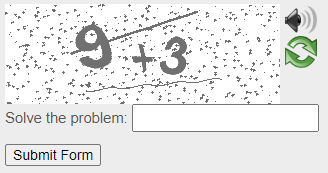
\includegraphics[width=6cm]{gfx/mygraphics/maths.png}}
    \qquad
    \subfloat[\centering]{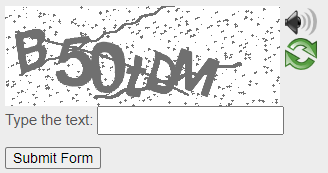
\includegraphics[width=6cm]{gfx/mygraphics/textbased.png}}
    \caption{Textbasierte CAPTCHAs aus der Securimage phpCaptcha Demo}   
    \label{fig:textbased}
\end{figure}

Anti-Segmentation Techniques zielen darauf ab, das Separieren der einzelnen Buchstaben durch Algorithmen zu erschweren. 
Um dies zu erreichen, gibt es verschiedene Herangehensweisen.
Eine von ihnen besteht daraus, dass nur die Konturen der verschiedenen Zeichen angezeigt werden, sodass diese nur von Menschen erkannt werden können,
Bots hingegen wenig Chancen haben, diese korrekt zu unterscheiden. Diese Art von CAPTCHA nennen \citeauthor{surveyofresearch} ``Hollow CAPTCHAs''. %Formulierung
Eine weitere Methode ist, Zeichen nah beieinander oder sogar überlappend darzustellen, 
was von \citeauthor{surveyofresearch} als ``crowing characters together $($CCT$)$ and overlapping'' bezeichnet wird.
Auch unruhige Hintergründe können Segmentierung behindern.
Ebenfalls beschrieben wird die Kombination von mehreren der beschriebenen CAPTCHAs zu einer ``two-layer'' Struktur,
wobei die Tatsache, dass es sich um mehrere Zeilen Text handelt, nicht erkannt werden kann. \cite[p.76]{surveyofresearch} \cite[p.132f]{Beheshti}

Anti-Recognition Techniques sind zum Beispiel verschiedene Schriftarten, die Rotation von Zeichen und ``Waving'', 
welche es erschweren, Zeichen als solche zu erkennen. 
Außerdem können in einigen Fällen auch sehr große Zeichensätze, beispielsweise Mandarin oder Japanisch, genutzt werden, 
wodurch das Finden von eindeutigen Lösungen erschwert werden kann.
Diese Techniken werden oftmals miteinander kombiniert.
\cite[p.77]{surveyofresearch}

Eine Kombination von Anti-Segmentation und Anti-Recognition Techniken ist in \autoref{fig:textbased} zu sehen.

\begin{figure}[h!]
    \centering
    \subfloat[\centering]{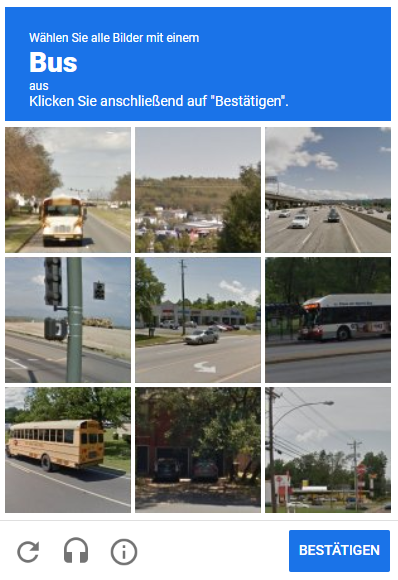
\includegraphics[width=6cm]{gfx/mygraphics/selectionbasedrecaptcha.png}}
    \qquad
    \subfloat[\centering]{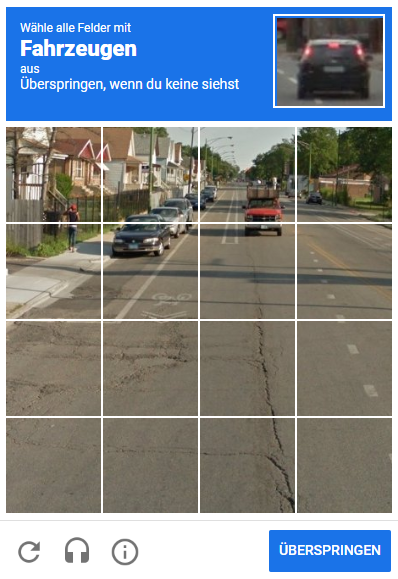
\includegraphics[width=6cm]{gfx/mygraphics/selectionbasedrecaptcha2.png}}
    \caption{Bildbasierte CAPTCHAs nach unzureichendem Score bei der Bewertung durch reCAPTCHA v2}   
    \label{fig:selectionbased}
\end{figure}

\subsubsection*{Bildbasierte CAPTCHA}
Es gibt verschiedene Arten von bildbasierten CAPTCHAs. 
Die wohl bekannteste ist ein in Quadrate aufgeteiltes Bild, wobei man jene Quadrate auswählen soll, welche einen bestimmten Gegenstand enthalten.
Eine Variation dieses CAPTCHAs besteht aus einer Zahl verschiedener Bilder, von denen eine Teilmenge ebenfalls ein gesuchtes Objekt beinhalten 
und sich semantisch ähneln. 
\autoref{fig:selectionbased} stellt diese Variationen dar.
In Abbildung \ref{fig:fortnite} sollen Hunde mit geschlossenen Augen ausgewählt werden,
was die Notwendigkeit der Zunahme der Komplexität dieser CAPTCHAs gut widerspiegelt. 
Außerdem kann auch auf das Erkennen von Gesichtern durch Menschen gesetzt werden.
Nähere Informationen zu genauen Techniken können in \cite[p.77ff]{surveyofresearch} nachgelesen werden.
Die beschriebenen ``selection-based CAPTCHA'' bezeichnen \citeauthor{surveyofresearch} als einfachste Form bildbasierter CAPTCHA. \cite[p.77]{surveyofresearch}

In Abbildung \ref{fig:genshin} sind zwei weitere Arten bildbasierter CAPTCHA dargestellt.
Links ist ein ``drag-based CAPTCHA'' zu sehen.
Hierbei werden Mausbewegungen, die Geschwindigkeit dieser Bewegungen
und die allgemeine Reaktionszeit überprüft.
Dies geschieht, wie in Abbildung \ref{fig:genshin} (a) zu sehen,
beispielsweise über das Verschieben eines Puzzleteils an die richtige Stelle.
Andere Variationen dieser CAPTCHA-Art verlangen, dass ein Bild mithilfe eines Schiebereglers in die richtige Position gebracht,
oder eine Kontur oder Bewegung mit der Maus nachverfolgt werden soll.
Auch hier kann in \cite[p.77]{surveyofresearch} genauer nachgelesen werden.

\begin{figure}[h!]
    \centering
    \subfloat[\centering]{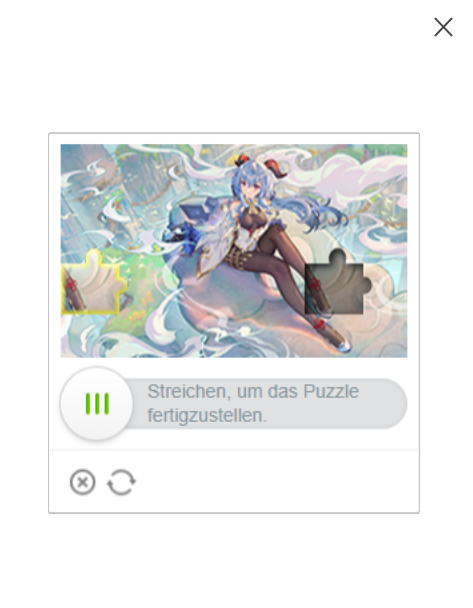
\includegraphics[width=6cm]{gfx/mygraphics/genshincaptcha.png}}
    \qquad
    \subfloat[\centering]{
\includegraphics[width=6cm]{gfx/mygraphics/hoyoversecaptcha.png}}
    \caption{Bildbasierte CAPTCHA von GeeTest bei Login in Genshin Impact $($a$)$ und dem Forum Hoyolab $($b$)$}   
    \label{fig:genshin}
\end{figure}

``Click-based CAPTCHA'' zeichnen sich dadurch aus, dass bestimmte Symbole oder Zeichen auf einem komplexen Hinter\-grund, 
teilweise auch in einer bestimmten Reihenfolge, angeklickt werden sollen.
Hierbei wird auf ``anti-detection'' und ``anti-recognition'' gesetzt. \cite[p.77]{surveyofresearch}

Ein Beispiel hierfür ist \ref{fig:genshin} (b).
Eine weitere Form der click-basierten CAPTCHAs sieht vor, dass Objekte ausgewählt werden sollen,
die beispielsweise die gleiche Textur besitzen oder räumlich nah an einem bestimmten anderen Objekt dargestellt sind. 
Diese sind zum Beispiel VTT\footnote[2]{VTT = Visual Turing Test} CAPTCHA. (Vgl. \cite[p.78]{surveyofresearch})

Ein Beispiel hierfür ist in \autoref{fig:geetest} zu sehen.
Hier wird über die Größe, Farbe und Position angegeben, welches Objekt angeklickt werden muss, um den CAPTCHA zu lösen.
Die Formulierung ``in front of'' ist hierbei auch auf Objekte bezogen, die nicht genau, sondern auch versetzt, vor dem gelben Zylinder stehen.
Zum Lösen des CAPTCHAs muss deshalb auf die grüne Kugel geklickt werden.

\begin{figure}[h!]
        \centering
        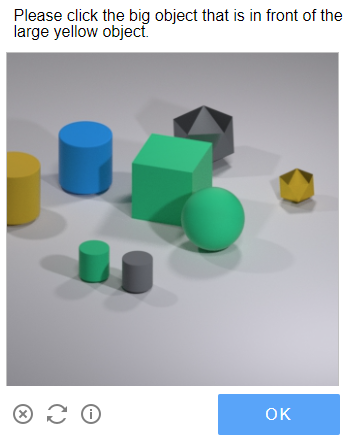
\includegraphics[width=6cm]{gfx/mygraphics/raeumlich.png} 
    \caption{Bildbasierter CAPTCHA aus der GeeTest Demo}
    \label{fig:geetest}
\end{figure}

\subsubsection*{Gamification}
Bei Gamification CAPTCHAs liegt der Fokus darauf, eventuell langwieriges Ausfüllen von CAPTCHAs so zu gestalten, dass Nutzer*innen dabei Spaß haben,
und es nicht als lästige Aufgabe ansehen.
\citeauthor{gamified} schreiben in ihrem Paper \citetitle{gamified} darüber, wie spielerisch lösbare CAPTCHAs die Nutzererfahrung verbessern können.
Hierbei werden Ideen wie das Ordnen von Cartoon-Panelen näher erläutert.
\pagebreak

Nicht nur lesen Nutzer*innen den Cartoon, sie wollen bei Fehlschlägen durch den Quizcharakter des CAPTCHAs die richtige Lösung in einem weiteren Versuch finden,
ohne über die Notwendigkeit der Wiederholung zur Verifizierung nachzudenken. \cite[p.41ff]{gamified}


\subsubsection*{Videobasierte CAPTCHA}
Eine weitere Form visueller CAPTCHAs sind videobasierte CAPTCHA. 
Nutzer*innen müssen beispielsweise verschiedene Bewegungen erkennen, die im Video ausgeführt werden,
oder auch angezeigte Werbung.
Dabei werden verschiedene Antwortmöglichkeiten vorgegeben, welche durch Raten auch durch Bots erfolgreich absolviert werden können.
Um dies zu umgehen gibt es Alternativen, die über das Beschreiben des gesehenen Videos funktionieren. \cite[p.79]{surveyofresearch} 

\subsubsection*{Audiobasierte CAPTCHA}
Als Alternative von visuellen CAPTCHAs können audiobasierte CAPTCHA genutzt werden.
Diese bieten sich vor allem für sehbehinderte Nutzer*innen an, welche bild- oder textbasierte CAPTCHA nur schwer oder gar nicht sehen und erkennen können.

Oft wird hier Text-To-Speech verwendet, wobei die gehörten Wörter durch die Nutzer*innen wiederholt werden sollen.
Eine weitere Möglichkeit ist das Abspielen bestimmter Töne, wie die einer Glocke oder eines Klaviers. 
Dies kann auch in Kombination mit verschiedenen Hintergrundgeräuschen angewandt werden, was das Erkennen eines bestimmten Tons für Roboter zusätzlich erschwert.
Außerdem gibt es Methoden, bei denen eine bestimmte Frage beantwortet werden muss, für die gesunder Menschenverstand notwendig ist. 
Beispielsweise kann nach einer Aussage wie ``Sally hat einen Nagel in den Boden gehämmert.'' gefragt werden, ob dieser Nagel vertikal oder horizontal war. \cite[p.3]{commonsense}

Neben Techniken, die hauptsächlich auf das Hören ausgelegt sind, kann der Fokus auch auf das Einsprechen von Phrasen durch die Nutzer*innen gelegt werden.
Es soll so erkannt werden, ob es sich um eine menschliche Stimme handelt.
\cite[p.78]{surveyofresearch}

\begin{figure}[h!]
    \centering
    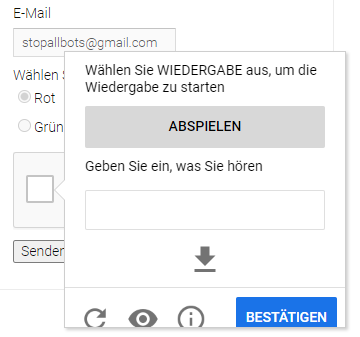
\includegraphics[width=6cm]{gfx/mygraphics/audio.png}
     \caption{Audiobasierte Alternative zu bildbasiertem CAPTCHA von reCAPTCHA v2}
      \label{fig:audio}
\end{figure}

\pagebreak

\subsection{Alternativen zu klassischen CAPTCHA}
\label{ch:basics:captcha:alternativen}
Neben klassischen Turing Tests gibt es weitere Möglichkeiten, Roboter und Menschen zu unterscheiden.
Aus diesem Grund werden nachfolgend Alternativen zu klassischen CAPTCHAs vorgestellt.

\subsubsection*{CAPTCHA mit minimalem User-Input}
Eine aktuell viel genutzte Form der Spam-Prävention ist reCAPTCHA v3 von Google. 
Hier werden keine klassischen Turing Tests durchgeführt. 
Vielmehr wird anhand verschiedener Faktoren bewertet, ob es sich um einen Bot oder einen Menschen handelt.
Die Betrachtung von Cookies oder der Häufigkeit von Anfragen durch die gegebene IP-Adresse werden hierbei unter anderem betrachtet.
In der Dokumentation wird angegeben, dass ein Score von 0.0 bis 1.0 vergeben werden kann. 
Hier gilt: Je niedriger der Score, desto wahrscheinlicher handelt es sich um einen Bot statt einer echten Nutzer*in. (Vgl. \cite{recaptchadoc})
Laut Google selbst soll reCAPTCHA v3 eine sehr gute Nutzererfahrung bieten, da es kaum bis gar keine Zuarbeit durch den Nutzer verlangt. \cite{googleblog:recaptcha}

ReCAPTCHA kann durch das Fehlen eines klassischen Turing Tests auch als eine CAPTCHA-Alternative interpretiert werden.

Ähnliche ``Invisible CAPTCHA''-Techniken werden auch von GeeTest \linebreak(\cite{geetest}) und hCaptcha (\cite{hcaptcha}) angeboten.

\begin{figure}[h!]
    \centering
\includegraphics[width=6cm]{gfx/mygraphics/recaptcha.png}
     \caption{CAPTCHA mit wenig benötigtem User-Input - reCAPTCHA v2}
      \label{fig:recaptcha}
\end{figure}

\pagebreak

Neben CAPTCHAs ohne jegliche Interaktion gibt es auch solche, 
die über das einfache Abhaken einer Checkbox verifizieren, ob es sich um einen Roboter handelt.
Eine andere Variation verlangt von den Nutzer*innen, dass ein Button angeklickt und gehalten werden soll. 

\subsubsection*{Honeypots}
Eine weitere Alternative zu klassischen CAPTCHA sind sogenannte Honeypots. 
Geprägt wurde der Begriff erstmals im Kalten Krieg, wo diese als Spionagetechnik eingesetzt wurde. \cite[p.2]{joshi:2011} 

Auch heute werden Honeypots eingesetzt, und zwar in der IT-Sicherheit. 
Oft werden sie mit Fallen assoziiert, welche Hacker anlocken sollen. 
Dadurch können Angriffsarten analysiert werden und echte Systeme werden nicht angegriffen.

Doch auch im Kontext der Unterscheidung von Menschen und Maschine gibt es Honeypots. 
So kann man HTML-Inputfelder durch CSS oder JavaScript verstecken, sodass diese nur durch Bots, welche den Quellcode der Seite scannen, ausgefüllt werden 
und nicht durch Menschen, da diese das Textfeld nicht sehen. 
Bei der Prüfung der Inputs kann nun überprüft werden, ob ein Bot in die Falle getappt ist. 
Nachzulesen sind solche Verfahren in verschiedenen Blogposts, wie \cite{perry:2019}.

\subsubsection*{Anti-Spam-Plugins}
Anti-Spam-Plugins können anstelle von CAPTCHAs genutzt werden, wenn man beispielsweise Kommentar\-bereiche moderieren möchte.
Das WordPress-Plugin ``Antispam-Bee'' arbeitet auf Basis verschiedener Anhaltspunkte, 
welche Auskunft darüber geben können, ob es sich bei Nutzer*innen wirklich um einen Menschen handelt.
Es kann beispielsweise überprüft werden, ob Kommentator*innen Gravatar
\footnote[3]{Gravatar steht für "Globally Recognized Avatar". 
Es kann ein Profilbild hochgeladen werden, welches mit einer oder mehreren E-Mail-Adressen verknüpft ist 
und neben Kommentaren angezeigt wird, wenn dort die entsprechende E-Mail-Adresse angegeben wurde. (Vgl. \cite{doku:antispambee})} nutzen.
Außerdem können IP-Adressen betrachtet werden und diese kann neben anderen Daten der Kommentator*innen gegebenenfalls in ``Spamdatenbanken'' gefunden werden.
Auch das Blockieren von Kommentaren aus bestimmten Ländern oder das Akzeptieren von Kommentaren in ausschließlich einer Sprache ist möglich.
Dieses Plugin und die beschriebenen Maßnahmen zur Spam-Präventionen sind nur eine von vielen Optionen, die hier zur Verfügung stehen.
\cite{blog:antispambee}
\cite{doku:antispambee}

\subsubsection*{Multi-Faktor-Authentifikation}
Die Authentifikation von Nutzer*innen über mehrere Schritte kann genutzt werden, um die unbefugte Nutzung von Accounts und Ähnlichem zu verhindern.
Dadurch kann beispielsweise verhindert werden, dass gestohlene Accountdaten für Spamangriffe genutzt werden können.

Dieser zweite Schritt, der vor dem Login durchgeführt werden muss, ist beispielweise das Anklicken eines Links oder das Eingeben eines Codes,
welcher über eine App oder SMS zugeschickt wurde.
Jedoch ersetzt dies nicht das Ausfüllen von CAPTCHAs.
Auch ein Algorithmus kann diese Aktionen mit Leichtigkeit ausführen. 
Die Nutzung von Multi-Faktor-Authentifikation ist zwar nicht schlecht,
bietet aber keine adäquate Alternative zu der Nutzung von CAPTCHAs. 
Aus diesem Grund wird die Multi-Faktor-Authentifi\-kation in Folgendem nicht weiter betrachtet.

\subsubsection*{Biometrie}
Eine relativ neue Art der Überprüfung von Nutzer*innen ist die Verifizierung durch Biometrie.
Hierbei wird über das Scannen des Gesichts oder die Erkennung einer Stimme entschieden, ob es sich wirklich um einen (bestimmten) Menschen handelt.
In \cite{rtcaptcha} wird diese Technik näher erläutert. 

Biometrische Verfahren werden hauptsächlich als eine Variation der Multi-Faktor-Authentifikation genutzt,
weshalb sie folgend nicht berücksichtigt werden. 

\section{User Experience}

User Experience (UX) beschreibt die Erfahrungen eines Users bei der Nutzung eines Systems. 
Das Ziel ist, diese Nutzererfahrung möglichst positiv zu halten. 
Im Kontext dieser Ausarbeitung wird die Definition des  ``international standard on ergonomics of human-system interaction'' $($ISO 9241-210$)$
aus dem Jahre 2010 verwendet. 
Diese definitiert UX als die Wahrnehmungen und Resonanzen einer Person, 
welche aus der $($voraussichtlichen$)$ Nutzung eines Produkts, Systems oder Services entstehen. \cite[p.1629]{berni_borgianni_2021}

Die Nutzererfahrung bei der Wahl und Nutzung von CAPTCHA ist neben der Sicherheit ein essentieller Bestandteil.
Bei der Entwicklung einer Bewertungsmatrix soll deshalb hier der Hauptfokus liegen.
Denn wenn ein CAPTCHA schwierig zu lösen ist, oder von bestimmten Personengruppen gar nicht bearbeitet werden kann, so stört dies nicht nur den Nutzungsfluss,
sondern führt gegebenenfalls auch dazu, dass Nutzer*innen die Seite verlassen, ohne ihre gewünschte Aktion zu vollenden. 

%\cite{surveyofresearch}

\chapter{Entwurf einer Bewertungsmatrix}
\label{ch:matrix}

Um die verschiedenen CAPTCHA-Arten bewerten zu können, muss eine Bewertungsmatrix entwickelt werden. 
Hierzu wird zuerst der Stand der Wissenschaft hinsichtlich bereits vorhandener Bewertungsmatrizen betrachtet 
und wie diese auf den vorliegenden Anwendungsfall anzuwenden sind. 

Anschließend werden die Kategorien Aufwand, also wie schwierig die Tests auszufüllen sind, Accessibility, technische Umsetzbarkeit 
und Sicherheit näher erläutert und es werden Fragen festgelegt, anhand derer man die Bewertung vornehmen kann.

Die gegebenen Kategorien wurden gewählt, um einerseits Fokus auf die verschiedenen Aspekte der Nutzererfahrung legen zu können,
andererseits jedoch auch nicht die Sicherheit als initialen Grund für die Verwendung von CAPTCHAs außer Acht zu lassen.

Um die Bewertung zu erleichtern, werden je Kategorien einige beispielhafte Leitfragen angegeben, welche bei Bedarf auch angepasst werden können.
In diesem Fall sollte dies jedoch für alle zu betrachtenden Techniken getan werden, um die Vergleichbarkeit zu gewährleisten.
Basierend auf diesen Fragen können Punkte von 0 bis 10 vergeben werden. 

\section{Stand der Wissenschaft}
\label{ch:matrix:sdw}

Es gibt bereits Methoden zur Bewertung von CAPTCHA.

In ihrem Paper ``A survey of research on CAPTCHA designing and breaking techniques'' beschreiben Zhang et al. das Design 
und mögliche Angriffe verschiedener CAPTCHA-Technologien – textbasiert, bildbasiert und audio-/videobasiert. 
Diese werden basierend auf „usability, robustness and their weaknesses and strengths“ bewertet. %(Zhang, et al., 2019, p. 75) 

``If the success rate of solving a CAPTCHA for humans is higher than 90\% and machines only achieve 
a success rate of less than 1\%, this CAPTCHA can be considered a good one $[$\dots$]$. 
Therefore, it is widely accepted that a good CAPTCHA is not only usable but also robust.'' %(Zhang, et al., 2019, p. 75) 
Quellen für diese Metrik sind Paper aus dem Jahre 2005 und 2008. 
Aus gleicher Quelle wird auch die Aussage gezogen, dass textbasierte CAPTCHA die meistgenutzte Art sei. 

%Da es sich bei Veröffentlichung bereits um ein 10 Jahre altes Paper handelte, ist the accuracy of this statement fragwürdig 
%(schreib das mal in normal wenn du denken kannst).
%Die Metrik zur Bewertung der CAPTCHA wird unzureichend erklärt imo, ich hab aber auch nicht alles gelesen lul

\section{Aufwand}
\label{ch:matrix:aufwand}

%Zeitbegrenzte CAPTCHA wtf???
%Leute klicken weg wenn es zu lange dauert / zu schwierig ist (diese seite mit der schlechten ux sehr gutes beispiel)
%Aufwändige implementierung in 4.4

\section{Accessibility}
\label{ch:matrix:accessibility}
Das Wörterbuch der Cambridge University definitiert Accessibility als ``$[$\dots$]$ the quality of being easy to understand $[$\dots$]$'' \cite{CACD:2008}

Dies stellt im Grunde auch die Definition für Accessibility im Kontext der zu entwickelnden Bewertungsmatrix dar: 

Wie leicht lassen sich die verschiedenen CAPTCHA-Arten verstehen? 

Sind sie für alle Personengruppen gleichermaßen nutzbar? 

Welche Probleme könnten auftreten?

Hierbei ist unter anderem zu beachten, dass CAPTCHA nicht nur an privaten PC-Arbeitsplätzen ausgefüllt werden, 
sondern auf verschiedensten Geräten und mit unterschiedlichen Gegebenheiten. 
Audiobasierte CAPTCHA können beispielsweise als störend wahrgenommen und deshalb nicht ausgefüllt werden, 
wenn das Abspielen von Tönen andere stören könnte $($in öffentlichen Verkehrsmitteln, in Büros, \dots$)$, 
oder das benutzte Gerät kann keinen Ton abspielen. Videobasierte CAPTCHA können eventuell nicht abgespielt werden, 
wenn das Internet schlecht ist.

Nicht zu vergessen sind verschiedene körperliche Einschränkungen von Nutzer*innen, 
die das Ausfüllen von CAPTCHAs erschweren oder gar unmöglich machen. Auch hier sind audiobasierte CAPTCHA zu erwähnen, 
da diese für schwerhörige oder gehörlose Menschen nicht absolvierbar sind. 

Ebenso müssen visuelle CAPTCHA für Screenreader optimiert werden, um sie für blinde Nutzer*innen nutzbar zu machen. 
Auch andere visuelle Beeinträchtigungen, wie beispielsweise Rot-Grün-Schwächen, müssen beachtet werden.

\section{Technische Umsetzbarkeit}
\label{ch:matrix:tu}

Bei der technischen Umsetzbarkeit wird das Augenmerk auf die Implementation und Instandhaltung der Techniken gelegt. 
Unzureichende Dokumentation kann die Implementation und eventuelles Debugging erheblich erschweren 
und spielt deshalb eine wichtige Rolle bei der Auswahl. 

Ist die Dokumentation ausreichend? Werden viele Ressourcen benötigt? Muss man vorhandenen Quellcode stark abändern?

\section{Sicherheit}
\label{ch:matrix:sicherheit}
Sicherheit ist der Hauptgrund für die Verwendung von Spam-Präventionstechniken. 
Wie bereits in den vorherigen Kapiteln erwähnt, werden CAPTCHAs und ihre Alternativen genutzt um bei dem Ausfüllen von Formularen Bots auszusortieren
und somit Spam zu vermeiden.
Es muss betrachtet werden, ob es schon Methoden zur Umgehung der CAPTCHAs gibt. 
Gibt es sogar bereits künstliche Intelligenzen, die bestimmte Tests lösen können?

\section{Berechnung einer Metrik}
\label{ch:matrix:berechnung}
Bei der Berechnung einer Metrik auf Basis der entworfenen Matrix muss eine korrekte Gewichtung gewählt werden. 
Diese ist nötig, um individuelle Entscheidungen für unterschiedliche Einsatzgebiete treffen zu können,
da die Bedürfnisse dieser stark unterscheiden können. 

Die Gewichtung für jede Kategorie wird anteilig von 100 Prozent angegeben.
So wird es ermöglicht, präzise und individuell zu priorisieren.




\chapter{Bewertung verschiedener Methoden}

Nachfolgend werden die verschiedenen Arten von CAPTCHA sowie einige Alternativen, wie Honeypots, Anti-Spam-Plugins, 
Multi-Faktor-Authentifikation und biometrische Verfahren auf Basis der zuvor entwickelten Matrix bewertet. 
Dafür wird sich an den in Kapitel \ref{ch:matrix} aufgestellten Leitfragen soweit möglich orientiert.

\section{Textbasierte CAPTCHA}
Durch ihren simplen Aufbau sind textbasierte CAPTCHAs relativ einfach zu verstehen.
Es sind wenige Clicks nötig, um einen solchen CAPTCHA auszufüllen. 
Bei optisch verzerrten Wörtern besteht jedoch die Möglichkeit, dass es zu Missverständnissen kommen kann.
So können beispielsweise ein kleines ``d'' und ein ``cl'' unter Umständen auch von Menschen verwechselt werden. 
In \autoref{fig:schwierig} ist ein ähnlicher Fall dargestellt. 
Wenn man sich nicht bewusst ist, dass hier nur korrekte Wörter der englischen Sprache erfragt werden,
kann das zweite Wort (``blotch'') auch als ``bbtch'' interpretiert werden.

\begin{figure}[h!]
    \centering
    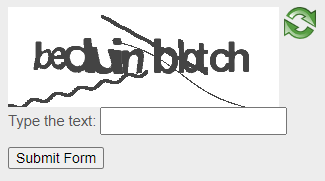
\includegraphics[width=6cm]{gfx/mygraphics/schwierig4.png}
    \caption{Textbasierter CAPTCHA aus der Securimage phpCaptcha Demo, welcher nicht eindeutig zu beantworten ist}
    \label{fig:schwierig}
\end{figure}

Damit würde der CAPTCHA nicht korrekt beantwortet werden können.
Diese Arten der textbasierten CAPTCHAs können gegebenenfalls nicht eindeutig beantwortet werden.
Aus diesem Grund kann bei der Bedienfreundlichkeit keine volle Punktzahl gegeben werden,
sondern es müssen je nach Komplexität ein bis zwei Punkte abgezogen werden.

Zeitliche Begrenzungen können vorkommen, sind aber nicht bei jeder Technik anzutreffen.
Hier ist, sofern gegeben, ebenfalls ein Punkt abzuziehen.

Accessability ist ambivalent zu betrachten.
Textbasierte CAPTCHA allein sind für sehbehinderte Menschen nicht nutzbar. 
Da dies eine Personengruppe vollständig ausschließt, werden zwei Punkte abgezogen.

Ebenso können die verschiedenen Techniken, die bei textbasierten CAPTCHAs angewandt werden, zu Problemen für Legastheniker führen.
Auch Menschen mit Farbfehlsichtigkeiten können durch eine Kombination von ungünstig generierten Hintergründen und Schriftfarben irritiert werden.
Aus diesem Grund wird auch hier jeweils ein Punkt abgezogen.

Einige textbasierte CAPTCHAs lassen sich gut audiobasiert umsetzen, 
um die Accessibility des CAPTCHAs zu gewährleisten. 
Dies würde somit nicht zu einem Punktabzug führen, wie es gegebenenfalls bei reinen audiobasierten CAPTCHAs (\autoref{ch:bewertung:audio}) der Fall wäre.

Die technische Umsetzbarkeit ist bei verschiedenen betrachteten Techniken zur Erstellung und Nutzung textbasierter CAPTCHAs sehr simpel gehalten.
Die Dokumentation ist gut und kann über Programmierschnittstellen (APIs) leicht eingebunden werden. (Vgl. \cite{hcaptcha} \cite{phpcaptcha} \cite{reallysimplecaptcha})
Aus diesem Grund kann hier die volle Punktzahl vergeben werden.

\citeauthor{surveyofresearch} schreiben in \citetitle{surveyofresearch}, 
dass Hollow CAPTCHA durch eine Kombination von Segmentierung und Recognition %TODO
mit einer Erfolgsrate von 36 bis 89 Prozent durch Bots gelöst werden konnten. (Vgl. \cite[p.76ff]{surveyofresearch}) %TODO

Ähnlich verhält es sich bei Überlappungen und CCT (``crowing characters together''):
Hier konnte bei verschiedenen Technologien mithilfe von unterschiedlichen Methoden
eine Erfolgsquote von 27,1 bis 53,2 Prozent erreicht werden. \cite[p.76]{surveyofresearch} %Quellen aus Text noch mit aufnehmen

Auch bei ``noise backgrounds'' und ``two-layer structures'' konnten solche Ergebnisse erzielt werden. 
(Vgl. \cite[p.76]{surveyofresearch})

Auf Basis dieser Erkenntnisse werden textbasierte CAPTCHAs wie in Tabelle \ref{table:matrix:text} bewertet.

%Multifonts, Rotation, Waving, Large character set \cite{surveyofresearch}

\begin{table}[h!]
    \caption{Bewertungsmatrix für textbasierte CAPTCHAs}
    \begin{center}
        \begin{tabular}{l|c}
            Kategorie                       & Bewertung \\\hline
            Bedienfreundlichkeit            & 7-9         \\
            Accessibility                   & 6        \\
            Technische Umsetzbarkeit        & 10         \\
            Sicherheit                      & 3-5         
        \end{tabular}
    \end{center}
    \label{table:matrix:text}
\end{table}

\section{Bildbasierte CAPTCHA}
Bildbasierte CAPTCHAs benötigen etwas mehr Aufwand als beispielsweise textbasierte CAPTCHAs.
Je nach verwendeter Technik muss auf eine Reihenfolge geachtet werden. 
Es ist auch möglich, dass bei einigen Bildern genau darauf geachtet werden muss, ob die gegebenen Antworten wirklich korrekt sind.
In \autoref{fig:fortnite} ist beispielsweise nur schwer zu erkennen, ob manche Hunde wirklich geschlossene Augen haben, 
oder ob der Kontrast zwischen Fell und Iris lediglich zu gering ist.

\begin{figure}[h!]
    \centering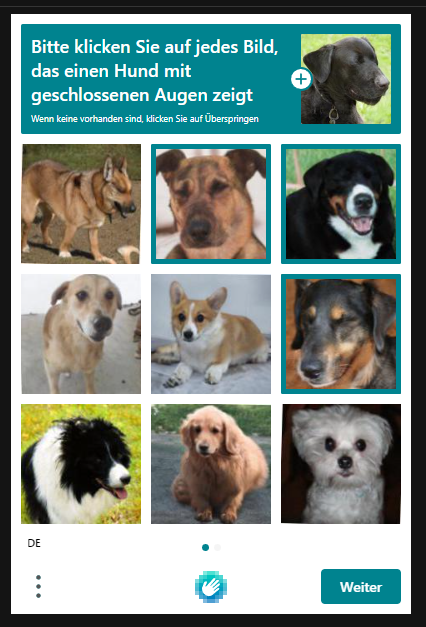
\includegraphics[width=6cm]{gfx/mygraphics/fuerfortnite.png}
 \caption{Bildbasierter CAPTCHA von hCaptcha bei Login auf der Epic Games Website}
      \label{fig:fortnite}
\end{figure}

Bei sehr detailreichen Bildern kann es vorkommen, dass auch ein Mensch mehrere Versuche benötigt, da eventuell nicht jedes gesuchte Objekt sofort erkannt wird.
Deshalb werden bei sehr hoher Komplexität oder bei schwer zu erkennenden Bildern zwischen 2 und 4 Punkte abgezogen werden.
Bei bildbasierten CAPTCHAs kommen zeitliche Begrenzungen eher selten vor. 

Auch hier besteht die Problematik, dass Menschen mit eingeschränker Sicht keine Chance haben, diese Art von CAPTCHAs adäquat auszufüllen.
Es gibt keine Möglichkeit, eine audiobasierte Alternative anzubieten. Durch diese schwerwiegende Einschränkung werden 5 Punkte abgezogen.
Doch auch für Menschen ohne Behinderung kann es, wie bereits erwähnt, schwierig sein, sie erfolgreich zu absolvieren.
Hier verschwimmen die Grenzen bei der Einschätzung des Aufwands und der Accessibility.

Die technische Umsetzbarkeit erfolgt bei bildbasierten CAPTCHAs ebenfalls über APIs. (Vgl. \cite{hcaptcha} \cite{arkoselabs} \cite{geetest})
Analog zu textbasierten CAPTCHAs kann deshalb volle Punktzahl vergeben werden.

Mithilfe einer Support Vector Machine konnte die CAPTCHA-Methode Asirra von Microsoft (Vgl. \cite{elson2007asirra})
mit einer Erfolgsrate von 82,7 Prozent absolviert werden. 
Die Nutzung von OpenCV ermöglicht, bestimmte Merkmale in Bildern algorithmisch zu analysieren.
Ebenso kann durch Trainieren von künstlichen Intelligenzen (KI) durch große Datenmengen (Deep Learning) eine hohe Erfolgsquote erreicht werden,
so konnten bereits mehrere CAPTCHAs von hochrangigen Unternehmen durch diese Weise erfolgreich erledigt durchgeführt werden.
Die Nutzung von KI ist noch nicht allzu weit verbreitet, gewinnt aber immer mehr an Bedeutung.
Da es bereits vermehrt sehr hohe Erfolgsquoten bei der Absolvierung von CAPTCHAs durch KIs und die Nutzung von OpenCV gab,
müssen für beide Techniken zur Umgehung dieser CAPTCHAs 2 Punkte abgezogen werden.
CAPTCHAs, welche über das Verschieben von Reglern funktionieren, sind durch ihr teilweise sehr aufwändiges Tracking von Mausbewegungen,
Reaktionszeit und anderen Metadaten etwas sicherer als selection-based CAPTCHAs. \cite[p.77f]{surveyofresearch}


\begin{table}[h!]
    \caption{Bewertungsmatrix für bildbasierte CAPTCHAs}
    \begin{center}
        \begin{tabular}{l|c}
            Kategorie                       & Bewertung \\\hline
            Bedienfreundlichkeit            & 6-10         \\
            Accessibility                   & 5        \\
            Technische Umsetzbarkeit        & 10         \\
            Sicherheit                      & 6         
        \end{tabular}
    \end{center}
\end{table}

\section{Videobasierte CAPTCHA}
Das Anschauen des jeweiligen Videos nimmt einige Sekunden in Anspruch und man muss dies je nach Komplexität wiederholen, 
da man eventuell nicht alle Aspekte bei dem ersten Durchlauf mitbekommt.
Wie ein Video als CAPTCHA auf Nutzer*innen wirken kann ist nicht genau festzulegen.
Einerseits handelt es sich dabei um etwas aufregenderes als einen simplen Text, andererseits kann dies auch schnell frustrieren.

Videobasierte CAPTCHAs brauchen eine schnelle Internetverbindung, um abgespielt werden zu können. %definiere gut
Desweiteren ist es nicht für jede Nutzer*in möglich zu erkennen, was genau im Video vor sich geht.
Dies führt dazu, dass videobasierte CAPTCHAs eine geringere Accessibility haben als dies bei anderen CAPTCHAs der Fall ist. 

Videobasierte CAPTCHA sind vergleichsweise wenig verbreitet. 
Ein bekannter Anbieter ist die Firma NuData Security mit NuCaptcha.
Nachdem \citeauthor{elie} in ihrem Blogartikel \citetitle{elie} darüber berichtete, 
dass NuCaptcha mit einer 90 prozentigen Erfolgsrate von einem Bot absolviert werden konnte,
wurden zwar einige Änderungen an NuCaptcha vorgenommen, jedoch existiert zum heutigen Tage keinerlei Dokumentation oder ähnliches für NuCaptcha.

Im Jahre 2015 gab es Verfahren, mit denen ein videobasiertes reCAPTCHA mit 31,75 prozentiger Erfolgsrate gebrochen werden konnte. 
Auch hier wirkt sich die Entwicklung besserer Bilderkennungstools und das Trainieren von KI negativ auf die Sicherheit aus.\cite[p.xx]{surveyofresearch}

Da videobasierte CAPTCHAs in der heutigen Zeit kaum noch von Bedeutung sind, werden diese nicht weiter betrachtet.
%\begin{table}[h!]
%    \caption{Bewertungsmatrix für videobasierte CAPTCHA}
%    \begin{center}
%        \begin{tabular}{l|c}
%            Kategorie                       & Bewertung \\\hline
%            Bedienfreundlichkeit            & 6         \\
%            Accessibility                   & 3        \\
%            Technische Umsetzbarkeit        & 2         \\
%            Sicherheit                      & 4         
%        \end{tabular}
%    \end{center}
%\end{table}

\section{Audiobasierte CAPTCHA}
\label{ch:bewertung:audio}

“Buster” ist ein Browser Addon, das reCAPTCHA audio challenges per speech recognition löst.
%
%A. Audio-based CAPTCHA
%This CAPTCHA is usually considered an alternative to a
%visual CAPTCHA in the case of visually impaired users [44].
%Users in most audio-based CAPTCHAs play the role of
%listeners, and they are required to complete the specified
%challenge based on what they have heard. A spoken
%CAPTCHA system was introduced in [45]. This system
%converts a selected word into speech using a Text-To-Speech
%(TTS) system, then plays the sound clip to users and asks them
%to say the word. In 2012, the SoundsRight audio CAPTCHA
%(Fig. 6(a)) provided in [48] asks users to identify a specific
%sound, such as the sound of a bell or a piano. This work has
%increased the success rates in audio Captchas from less than
%50% to over 90% for blind users. Meutzner et al. presented a
%new type of audio CAPTCHA [50] that uses additional
%nonsense speech sounds that are confusing for speech
%recognizers, while being less critical for human listeners. In
%2016, they also proposed a nonspeech audio CAPTCHA [61],
%which is entirely based on the classification of sound events
%mixed into an environmental scene. Moreover, the HuMan
%CAPTCHA designed in [60] asks users to answer the
%presented questions by combining ambient noise and common
%sense knowledge. There is another type of audio-based
%CAPTCHA in which users play the role of speakers and are
%required to pronounce rather than simply listen. For instance,
%Gao et al. [47] proposed a new sound-based CAPTCHA (Fig.
%6(b)) that exploits the differences between a human voice a
%synthetic voice. A user is required to read out a given sentence
%rather than listening an audio file.
%Fig. 6. Examples of audio-based CAPTCHAs
%Attack and defense always go together. A two-stage attack
%for the listener model can always obtain a good attack result.
%In detail, the audio-based CAPTCHA is segmented into
%several regions regarding the location of each spoken word
%first. Then, the regions are recognized by automatic speech
%recognition programs. Tam et al. achieved success rates of up
%to 71% (Google Audio CAPTCHA, reCAPTCHA Audio
%CAPTCHA, Digg CAPTCHA)[44]. Bursztein et al. achieved
%success rates of 45%, 49% and 83% on the CAPTCHAs of
%Yahoo, Microsoft and eBay, respectively[49]. Some
%78
%Authorized licensed use limited to: Fachhochschule FH Darmstadt. Downloaded on July 29,2022 at 08:34:41 UTC from IEEE Xplore. Restrictions apply.
%researchers have even proposed that most of the digit-based
%audio CAPTCHAs are successfully broken with success rates
%between 50%-90% [44][52][54].


\begin{table}[h!]
    \caption{Beispielhafte Bewertungsmatrix}
    \begin{center}
        \begin{tabular}{l|c}
            Kategorie                       & Bewertung \\\hline
            Bedienfreundlichkeit                         & 7         \\
            Accessibility                   & 10        \\
            Technische Umsetzbarkeit        & 3         \\
            Sicherheit                      & 9         
        \end{tabular}
    \end{center}
\end{table}

\begin{table}[h!]
    \caption{Beispielhafte Bewertungsmatrix}
    \begin{center}
        \begin{tabular}{l|c}
            Kategorie                       & Bewertung \\\hline
            Bedienfreundlichkeit                         & 7         \\
            Accessibility                   & 10        \\
            Technische Umsetzbarkeit        & 3         \\
            Sicherheit                      & 9         
        \end{tabular}
    \end{center}
\end{table}

\section{Gamification}

\begin{table}[h!]
    \caption{Beispielhafte Bewertungsmatrix}
    \begin{center}
        \begin{tabular}{l|c}
            Kategorie                       & Bewertung \\\hline
            Bedienfreundlichkeit                         & 7         \\
            Accessibility                   & 10        \\
            Technische Umsetzbarkeit        & 3         \\
            Sicherheit                      & 9         
        \end{tabular}
    \end{center}
\end{table}

\section{Alternativen zu CAPTCHA}

\subsection{Honeypot}

\begin{table}[h!]
    \caption{Beispielhafte Bewertungsmatrix}
    \begin{center}
        \begin{tabular}{l|c}
            Kategorie                       & Bewertung \\\hline
            Bedienfreundlichkeit                         & 7         \\
            Accessibility                   & 10        \\
            Technische Umsetzbarkeit        & 3         \\
            Sicherheit                      & 9         
        \end{tabular}
    \end{center}
\end{table}

\subsection{Anti Spam Plugins}

\begin{table}[h!]
    \caption{Beispielhafte Bewertungsmatrix}
    \begin{center}
        \begin{tabular}{l|c}
            Kategorie                       & Bewertung \\\hline
            Bedienfreundlichkeit                         & 7         \\
            Accessibility                   & 10        \\
            Technische Umsetzbarkeit        & 3         \\
            Sicherheit                      & 9         
        \end{tabular}
    \end{center}
\end{table}

\subsection{Multi-Faktor Authentifikation}

\begin{table}[h!]
    \caption{Beispielhafte Bewertungsmatrix}
    \begin{center}
        \begin{tabular}{l|c}
            Kategorie                       & Bewertung \\\hline
            Bedienfreundlichkeit                         & 7         \\
            Accessibility                   & 10        \\
            Technische Umsetzbarkeit        & 3         \\
            Sicherheit                      & 9         
        \end{tabular}
    \end{center}
\end{table}

\subsection{Biometrie}

\begin{table}[h!]
    \caption{Beispielhafte Bewertungsmatrix}
    \begin{center}
        \begin{tabular}{l|c}
            Kategorie                       & Bewertung \\\hline
            Bedienfreundlichkeit                         & 7         \\
            Accessibility                   & 10        \\
            Technische Umsetzbarkeit        & 3         \\
            Sicherheit                      & 9         
        \end{tabular}
    \end{center}
\end{table}
\chapter{Empfehlungen}
\label{ch:empfehlung}

Basierend auf den im vorherigen Kapitel aufgestellten Bewertungen werden für verschiedene fiktive Szenarien Scores berechnet 
und mithilfe dieser Empfehlungen hinsichtlich der Wahl des CAPTCHA ausgesprochen. 
Dies soll einerseits als Beispiel zur Anwendung dienen, 
andererseits auch eine erste Orientierung bei der Auswahl der zu prüfenden Techniken geben. 
Erwartet wird, dass trotz eindeutiger Bewertungen in \autoref{ch:bewertung} durch unterschiedliche Gewichtigungen
individuelle Empfehlungen ausgesprochen werden können. 
Dabei sollen die errechneten Scores positive und negative Eigenschaften der einzelnen CAPTCHA-Arten wiederspiegeln.

\subsubsection*{Beispiel 1 - Bank}
Als erstes Szenario soll eine Bank dienen, die für ihr Online Banking mit CAPTCHAs arbeitet.
Sicherheit ist hier besonders wichtig, 
da eine Störung des Systems fatal für Kund*innen und die Bank selbst sein könnte.
Außerdem sollte möglichst allen Kund*innen der Zugriff möglich sein, 
weshalb Accessability ebenfalls eine große Rolle spielt.
Aus diesem Grund kann in Sachen Bedienfreundlichkeit 
und auch bei der technischen Umsetzbarkeit zu Gunsten der Ausfallsicherheit verzichtet werden.
Daraus ergeben sich folgende Gewichtungen:

\begin{table}[h!]
    \caption{Gewichtung für Beispiel 1}
    \begin{center}
        \begin{tabular}{l|c}
            Kategorie                       & Gewichtung \\\hline
            Bedienfreundlichkeit            & 15\%         \\
            Accessibility                   & 30\%        \\
            Technische Umsetzbarkeit        & 15\%         \\
            Sicherheit                      & 40\%         
        \end{tabular}
    \end{center}
\end{table}

In \autoref{tabellen1} sind die ausführlichen Bewertungsmatrizen für Beispiel 1 zu finden. 
Aus diesen Tabellen lassen sich folgende Bewertungen entnehmen.

Aus den vorliegenden Ergebnissen lässt sich erkennen, dass Invisible \linebreak CAPTCHAs die höchste Gesamtnote erreichen konnten.
Insbesondere bei der Accessibility können sie überzeugen, 
da sie durch ihr Arbeiten im Hintergrund keine Interaktion verlangen und somit von allen Nutzer*innen problemlos benutzt werden können.
Außerdem sind CAPTCHAs mit wenig User-Input relativ sicher, da fast ausschließlich Metadaten betrachtet werden und das genaue Verfahren unbekannt ist.
Dadurch ist es schwerer, diese Daten für Bots nachzustellen.

Ähnlich verhält es sich im Best Case bei bildbasierten CAPTCHAs, besonders wenn hier Mausbewegungen und Ähnliches mit in Betracht gezogen werden.
Zwar ist hier die direkte Mitarbeit der Nutzer*innen nötig, jedoch handelt es sich im besten Fall um wenige Klicks. 

Es kann jedoch auch vorkommen, dass der bildbasierte CAPTCHA sehr kompliziert oder unverständlich ist und mehrere Versuche notwendig sind,
weshalb sie nicht die beste Wahl sind.
Außerdem ist es durch verschiedene Algorithmen zur Bildbearbeitung und den Einsatz von künstlicher Intelligenz möglich,
eine Vielzahl von Objekten korrekt zu erkennen.

Auch Honeypots erzielen einen relativ hohen Score.
Dies liegt daran, dass sie ebenfalls mit sehr wenig Nutzerinteraktion verbunden sind
und dementsprechend auch wenig Probleme im Bereich der Accessibility bereiten.
Hier besteht jedoch das Problem, dass ein einmal erkannter Honeypot bei jedem weiteren Versuch umgangen werden kann.
Damit wird das System schlagartig wesentlich anfälliger für Spam-Angriffe, da der Sicherheitsmechanismus nicht mehr zuschlagen kann.
Aus diesem Grund sind Honeypots nicht zu empfehlen, wenn es sich um Systeme handelt, die eine sehr hohe Sicherheit verlangen.

Audiobasierte CAPTCHAs konnten keine hohe Gesamtnote erreichen.

Dies hängt unter anderem mit ihrer geringen Bewertung im Bereich Accessibility zusammen,
da sie zwar als Alternative zu visuellen CAPTCHAs sehr gut funktionieren, jedoch als alleinige Lösung einige Probleme mit sich bringen.
So schließen sie nicht nur gehörlose Menschen gänzlich aus, sondern können auch hörende Menschen den CAPTCHA eventuell nicht absolvieren,
da sie sich in Situationen befinden, in denen sie keine Töne abspielen wollen oder (technisch) können.

Textbasierte CAPTCHAs erzielen im Worst Case den niedrigsten Score, doch auch im Best Case sind sie auf dem vorletzten Platz.
Dies liegt unter anderem an der niedrigen Bewertung im Bereich der Sicherheit, 
da es hier viele Methoden gibt, textbasierte CAPTCHAs durch Algorithmen erkennen und lösen zu lassen.
Auch im Bereich der Accessibility muss darauf geachtet werden, dass es ausreichend Alternativen für Menschen gibt,
die Probleme mit visuellen CAPTCHAs haben könnten.

Eine Kombination verschiedener CAPTCHA-Arten, wie es beispielsweise bei reCAPTCHA oder hCaptcha der Fall ist, 
kann eventuelle Mängel bei einzelnen Techniken beheben.

Oftmals werden bildbasierte CAPTCHAs als Backup für Invisible CAPTCHA verwendet, sollten die Metadaten keine genauen Schlüsse zulassen.
Das Anbieten von audiobasierten CAPTCHAs als weitere Option zu einem visuellen CAPTCHA ist ebenfalls zu empfehlen.
So kann eine maximale Accessibility erreicht werden.

Im Bereich der Sicherheit ist vor allem darauf zu achten, stets die neuste Version des gewählten CAPTCHAs zu nutzen 
und sich über eventuelle Sicherheitslücken zu informieren.

\begin{table}[h!]
    \caption{Bewertungen für Beispiel 1}
    \begin{center}
        \begin{tabular}{l|c}
            CAPTCHA-Art                       & Gesamtnote \\\hline
            textbasiert            &  5.55-7.85       \\
            bildbasiert                   &  6.3-8.4      \\
            audiobasiert        & 5.75-5.9         \\
            invisible*                      & 9.05         \\
            Honeypots       & 7.55\\
            \multicolumn{2}{l}{\footnotesize * Invisible steht hier für jegliche CAPTCHAs} \\
            \multicolumn{2}{l}{\footnotesize \space \space mit minimalem User-Input}
        \end{tabular}
    \end{center}
\end{table}

\subsubsection*{Beispiel 2 - Forum}
Das zweite Szenario soll ein kleines Internetforum sein, in dem ein CAPTCHA ausgefüllt wird, bevor ein Beitrag veröffentlicht wird.
Hierbei ist besonders auf die Bedienfreundlichkeit zu achten, damit Nutzer*innen sich mit möglichst wenig Irritation austauschen können.
Außerdem soll die gewählte Technologie möglichst einfach technisch umzusetzen sein, um Kosten und Ressourcenverbrauch gering halten zu können.
Accessibility ist zwar auch von Relevanz, jedoch nicht so stark wie zuvor genannte Kategorien, da dieses Forum nicht unbedingt von jeder Person genutzt werden können soll.
Die Sicherheit ist aufgrund der geringen Anzahl an abgegebenen Beiträgen vergleichsweise unwichtig.
Sollten viele Nachrichten durch Bots veröffentlicht werden, können diese durch Administrator*innen leicht wieder entfernt werden.

\begin{table}[h!]
    \caption{Gewichtung für Beispiel 2}
    \begin{center}
        \begin{tabular}{l|c}
            Kategorie                       & Gewichtung \\\hline
            Bedienfreundlichkeit            & 35\%         \\
            Accessibility                   & 20\%        \\
            Technische Umsetzbarkeit        & 35\%         \\
            Sicherheit                      & 10\%         
        \end{tabular}
    \end{center}
\end{table}

Analog zu Beispiel 1 sind die genauen Bewertungsmatrizen in \autoref{tabellen2} hinterlegt.
Es ergeben sich folgende Gesamtnoten:

\begin{table}[h!]
    \caption{Bewertungen für Beispiel 2}
    \begin{center}
        \begin{tabular}{l|c}
            CAPTCHA-Art                       & Gesamtnote \\\hline
            textbasiert            & 7.45-9.15        \\
            bildbasiert                   & 7.2-9.6       \\
            audiobasiert        & 7.25-7.4         \\
            invisible*                      & 9.45         \\
            Honeypots & 8.95 \\
           \multicolumn{2}{l}{\footnotesize * Invisible steht hier für jegliche CAPTCHAs} \\
           \multicolumn{2}{l}{\footnotesize   \enspace mit minimalem User-Input}
        \end{tabular}
    \end{center}
\end{table}

Auch hier erreichen CAPTCHAs mit geringem User-Input eine sehr gute Bewertung.
Die höchste Gesamtnote erreichen im Best Case jedoch bildbasierte CAPTCHAs.

Es ist zu beachten, dass es sich hier nur um eine Diskrepanz von 0.3 Notenpunkten handelt. 
Sie entsteht dadurch, dass bei bildbasierten CAPTCHAs weniger Interaktion nötig sein kann als bei einem invisible CAPTCHA,
welcher aufgrund eines zu niedrigen Scores zusätzliche Verifikation, 
wie das Lösen eines bild- oder audiobasierten CAPTCHAs, benötigt.
Im Bereich der technischen Umsetzbarkeit können beide Methoden voll überzeugen. 
Die Nutzung von APIs ermöglicht eine schnelle Implementation.

Textbasierte CAPTCHAs erzielen im Best Case ebenfalls eine hohe Punktzahl. 
Dies liegt daran, dass besonders der Punkt Sicherheit keine große Rolle spielt
und die niedrige Bewertung die Gesamtnote deshalb nicht so stark beeinflusst wie es bei Beispiel 1 der Fall ist. 

Durch die große Spannweite in den Kategorien Bedienfreundlichkeit und Accessibility
liegen die Bewertungen des Worst Case und Best Case bei textbasierten CAPTCHAs weit auseinander.
Hier ist es also stark von der Einzellösung abhängig, ob diese wirklich eine gute Wahl für diesen Anwendungsfall darstellen würde.

Ähnlich verhält es sich auch bei bildbasierten CAPTCHAs. 

Auch Honeypots bilden eine gute Alternative. 
Da die Sicherheit in diesem Beispiel nur gering gewertet wird, ist die Problematik, dass sobald ein Honeypot erkannt wurde,
kein Schutz mehr besteht, nicht allzu relevant. 
In Sachen Bedienfreundlichkeit und Accessability verhalten sich Honeypots analog zu invisible CAPTCHAs,
jedoch ohne eventuell benötigte zusätzliche Verifikation.

Audiobasierte CAPTCHAs können trotz ihrer relativ hohen Bedienfreundlichkeit und technischer Umsetzbarkeit keinen hohen Score erzielen.
Das liegt daran, dass sie eine sehr niedrige Bewertung in den Kategorien Accessability und Sicherheit haben,
was sich trotz ihrer vergleichsweise niedrigen Bewertung stark auf die Gesamtnote auswirkt.

Gewählt werden sollte hier ein CAPTCHA, das möglichst einfach auszufüllen ist, wie insivible CAPTCHAs oder bildbasierte CAPTCHAs. 
Honeypots können aufgrund ihrer hohen Bedienfreundlichkeit ebenfalls genutzt werden, 
sind technisch jedoch etwas schwieriger umzusetzen als andere Methoden.
\chapter{Bewertung der Ergebnisse}

Die zuvor beschriebenen Bewertungen dienen lediglich als Orientierung, 
bei Benutzung der entwickelten Matrix sollten diese individuell neu durchgeführt werden,
da je nach Bedarf die vorgegebenen Leitfragen abgeändert oder anders interpretiert werden können.
Dadurch entsteht ein gewisser Grad an Subjektivität, welcher sich nicht vermeiden lässt.
Insbesondere bei der Bewertung der technischen Umsetzung muss individuell nachjustiert werden,
da die Gegebenheiten sehr individuell sein können und man beispielsweise von einer im Allgemeinen guten Dokumentation nicht auf Einzelfälle schließen kann.
\chapter{Fazit}

Mithilfe der entwickelten Matrix können verschiedene CAPTCHA-Techno\-logien entweder selbst bewertet werden,
oder es kann die in \autoref{ch:bewertung} abgegebene Einschätzung verwendet werden.
Durch eine angemessene Gewichtung je nach Anwendungsfall können die betrachteten Arten miteinander verglichen werden.

Neben der Betrachtung der allgemeinen CAPTCHA-Arten kann die Matrix auch für spezifische Produkte angewandt werden,
sodass auch diese miteinander verglichen werden können.

ReCAPTCHA ist momentan die beste Wahl, da es meist wenig oder keinen User-Input benötigt.
Dies wird auch dadurch bestätigt, dass einige andere Techniken gar nicht mehr anzutreffen sind,
wie Gamification oder videobasierte CAPTCHA. 
Die hohe Anzahl der Webseiten, die reCAPTCHA nutzen, bestätigen diese Annahme. \cite{stats}

Wie bereits in \autoref{ch:bewertungergebnisse} erwähnt, gibt es hier jedoch Bedenken bei der Datensicherheit.
Aus diesem Grund sollten auch Alternativen in Betracht gezogen werden. 

Die entwickelte Bewertungsmatrix kann auch für andere Arten von Software genutzt werden,
wenn die angegebenen Leitfragen entsprechend angepasst werden. 
\chapter{Ausblick}

Künstliche Intellligenzen bewegen sich immer näher darauf hin, Turing Tests bestehen zu können.
Bereits 2014 behauptete Kevin Warwick, dass der Chatbot ``Eugene Goostman'' den Turing Test bestanden hätte,
da dieser von 33\% seiner Chatpartner bei einem Event davon überzeugen konnte, ein Mensch zu sein. \cite{eugene}

Im Zuge dieser stetigen Entwicklung müssen auch CAPTCHAs weiterentwickelt werden,
um nicht obsolet zu werden. 

Dies hat zur Folge, dass CAPTCHAs sich in zwei Richtungen bewegen können:

Einerseits müssen klassische visuelle oder audiobasierte CAPTCHAs stetig komplizierter gestaltet werden,
um vorhandenen Algorithmen zur Bild- und Spracherkennung entgegenwirken zu können.

Andererseits kann auch vermehrt auf Metadaten und Ähnliches zurückgegriffen werden, was eventuelle Datenschutzeinschränkungen zur Folge hat.

Als Lösung für dieses Problem werden schon heute die verschiedenen CAPTCHA-Arten miteinander kombiniert.
Ist sich beispielsweise reCAPTCHA oder hCaptcha nicht sicher, ob es sich bei der Nutzer*in um einen Menschen handelt,
müssen weitere CAPTCHAs ausgefüllt werden.

Neben der Nutzung von vorhandenen Produkten auf dem Markt können bei Bedarf auch eigene CAPTCHAs entwickelt werden.
Dies gestaltet sich jedoch aufgrund der bereits genannten Entwicklungen stetig komplizierter.

Die Grenze, wann etwas noch als CAPTCHA bezeichnet werden kann, vist schwierig zu ziehen.
So handelt es sich bei invisible CAPTCHAs auch nicht um klassische Tests mit Nutzereingaben.

Eventuell gibt es deshalb in Zukunft eine neue Bezeichnung inklusive neuer Definition, welche CAPTCHAs ablösen könnte.
%\include{chapters/examples/chapter01}
%\include{chapters/examples/chapter02}
%\include{chapters/examples/chapter03}
%*************************************************************************
% Recommendations
%*************************************************************************
%\part{Empfehlungen zur Erstellung wissenschaftlicher Abschlussarbeiten}
%\label{pt:recommendations}
%*************************************************************************
% Backmatter
%*************************************************************************
\appendix
%\renewcommand{\thechapter}{\alph{chapter}}
\cleardoublepage
\part{Appendix}
%\include{chapters/examples/appendix01}
%\include{chapters/examples/appendix02}
%*************************************************************************
% Other Stuff in the Back
%*************************************************************************
\cleardoublepage\include{frontbackmatter/Bibliography}
%*************************************************************************
% Game Over: Restore, Restart, or Quit?
%*************************************************************************
\end{document}
%*************************************************************************
